% Created 2022-04-20 Wed 09:38
% Intended LaTeX compiler: pdflatex
\documentclass[smaller]{beamer}\usepackage{listings}
\usepackage{color}
\usepackage{amsmath}
\usepackage{array}
\usepackage[T1]{fontenc}
\usepackage{natbib}
\lstset{
keywordstyle=\color{blue},
commentstyle=\color{red},stringstyle=\color[rgb]{0,.5,0},
literate={~}{$\sim$}{1},
basicstyle=\ttfamily\small,
columns=fullflexible,
breaklines=true,
breakatwhitespace=false,
numbers=left,
numberstyle=\ttfamily\tiny\color{gray},
stepnumber=1,
numbersep=10pt,
backgroundcolor=\color{white},
tabsize=4,
keepspaces=true,
showspaces=false,
showstringspaces=false,
xleftmargin=.23in,
frame=single,
basewidth={0.5em,0.4em},
}
\usepackage{natbib, dsfont, pgfpages, tikz,amssymb, amsmath,xcolor}
\bibliographystyle{abbrvnat}
% New operators and commands
\newcommand{\Z}{\mathbb{Z}}
\newcommand{\Q}{\mathbb{Q}}
\newcommand{\R}{\mathbb{R}}
\newcommand{\N}{\mathbb{N}}
\newcommand{\C}{\mathbb{C}}
\renewcommand{\S}{\mathbb{S}}
\newcommand{\blank}{\makebox[1ex]{\textbf{$\cdot$}}}
\newcommand\independent{\protect\mathpalette{\protect\independenT}{\perp}}
\def\independenT#1#2{\mathrel{\rlap{$#1#2$}\mkern2mu{#1#2}}}
\renewcommand{\phi}{\varphi}
\renewcommand{\epsilon}{\varepsilon}
\newcommand*\diff{\mathop{}\!\mathrm{d}}
\newcommand{\weakly}{\rightsquigarrow}
\newcommand\smallO{
  \mathchoice
    {{\scriptstyle\mathcal{O}}}% \displaystyle
    {{\scriptstyle\mathcal{O}}}% \textstyle
    {{\scriptscriptstyle\mathcal{O}}}% \scriptstyle
    {\scalebox{.6}{$\scriptscriptstyle\mathcal{O}$}}%\scriptscriptstyle
}
\newcommand{\midd}{\; \middle|\;}
\newcommand{\1}{\mathds{1}}
\usepackage{ifthen} %% Empirical process with default argument
% \newcommand{\G}[1][]{%
%    \ifthenelse{ \equal{#1}{} }
%       {\ensuremath{\mathbb{G}_n}}
%       {\ensuremath{\mathbb{G}_{#1}}}
% }
% New version:
\newcommand{\G}[2][n]{
{\ensuremath{\mathbb{G}_{#1}}{\left[#2\right]}}
}
\DeclareMathOperator*{\argmin}{\arg\!\min}

% New operators for consistent notation
\newcommand{\V}{\mathrm{Var}} % variance
\newcommand{\measure}[1]{\mathrm{{#1}}} % measure
% \newcommand{\measure}[1]{\textnormal{\textbf{{#1}}}} % measure
\newcommand{\m}[1]{\measure{#1}} % measure shortcut
\newcommand{\eqd}{\stackrel{d}{=}} % equality in distribution
\newcommand{\arrow}[1]{\xrightarrow{\; {#1} \;}}
\newcommand{\arrowP}{\xrightarrow{\; \m{P} \;}} % convergence in probability
\newcommand{\leb}{\lambda} % the Lebesgue measure
\newcommand{\T}{\top} % transpose
\newcommand{\KL}{\ensuremath{D_{\mathrm{KL}}}}

\usepackage{xargs}
% Make it easy to change counterfactual notation:
\newcommandx{\cf}[4][3={}, 4={}]{
  % \ifthenelse{ \equal{#4}{} }
  % {{#1^{#2}}(#3)}
  {\ifthenelse{ \equal{#3}{} }
    {{#1^{#2}}_{#4}}
    {{#1^{#2}}_{#4}(#3)}}
}

% Easily change notation:
\DeclareMathOperator{\TT}{\Psi} % target parameter
\newcommand{\lp}{\mathcal{L}_{\P}^2} % shortcut for lp2 space
\newcommand{\empmeas}{\hat{\mathbb{P}}_n} % empirical measure
\DeclareMathOperator{\E}{\mathbb{E}} % expectation
\renewcommand{\P}{\m{P}} % probability
\newcommand{\ic}{\mathrm{IF}} % influence curve
\setbeamertemplate{footline}[frame number]
\beamertemplatenavigationsymbolsempty
\usepackage{appendixnumberbeamer}
\setbeamercolor{gray}{bg=white!90!black}
\setbeamertemplate{itemize items}{$\circ$}

\renewcommand*\familydefault{\sfdefault}
\itemsep2pt
\usepackage[utf8]{inputenc}
\usepackage[T1]{fontenc}
\usepackage{graphicx}
\usepackage{longtable}
\usepackage{wrapfig}
\usepackage{rotating}
\usepackage[normalem]{ulem}
\usepackage{amsmath}
\usepackage{amssymb}
\usepackage{capt-of}
\usepackage{hyperref}
\usetheme{default}
\author{Anders Munch}
\date{\today}
\title{Journal club -- Models as Approximations}
\begin{document}

\maketitle
\section{The paper}
\label{sec:org2f1197a}
\begin{frame}[label={sec:orgbf567e2}]{The paper}
\hfill

\begin{center}
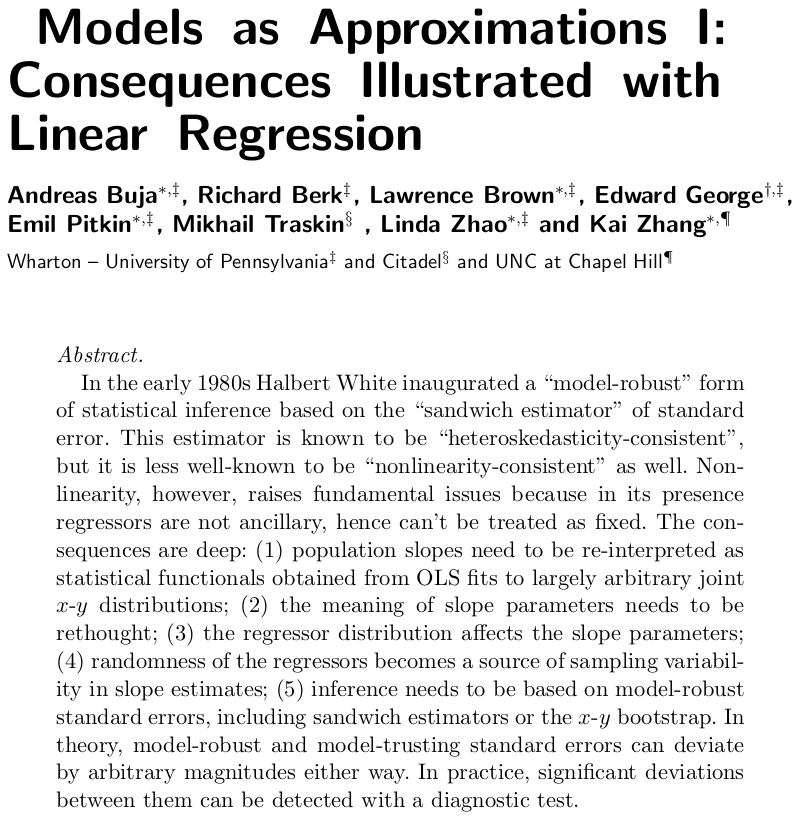
\includegraphics[width=.9\linewidth]{./quotes/abstract.png}
\end{center}
\end{frame}

\begin{frame}[label={sec:org410afd0}]{Discussion paper}
\begin{itemize}
\item Memorial Issue of \emph{Statitical Science} for Lawrence D. Brown
\item Paper in two parts: Special case of linear regression (part I, \cite{buja2019models}) and general
case (part II, \cite{buja2019models2}). Part II defines a notion of ``well-specification for
regression functionals'' and propose diagnostic tools.
\end{itemize}
\hfill

\begin{block}{Comments by}
\begin{itemize}
\item \citeauthor*{ghanem2019discussion} (UC Davis and Washington University in St. Louis)
\item \citeauthor*{rinaldo2019comment} (Carnegie Mellon University, Pittsburgh)
\item \citeauthor*{whitney2019comment} (Imperial College London, University of Washington, Seattle)
\item and others.
\end{itemize}
\end{block}
\end{frame}

\begin{frame}[label={sec:orgec21af0}]{Overall idea}
Understand what is estimated with linear a linear regression (or more general M-estimators) when the
model is mis-specified. 

\hfill

Define the parameter \(\beta\) as a functional defined on the data distribution \(P \in \mathcal{P}\):

\hfill

\begin{center}
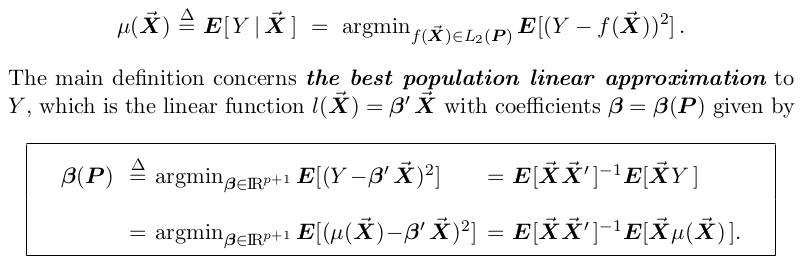
\includegraphics[width=.9\linewidth]{./quotes/sect3-main-def.png}
\end{center}
\end{frame}

\begin{frame}[label={sec:org8b4dc49}]{One consequence}
\begin{center}
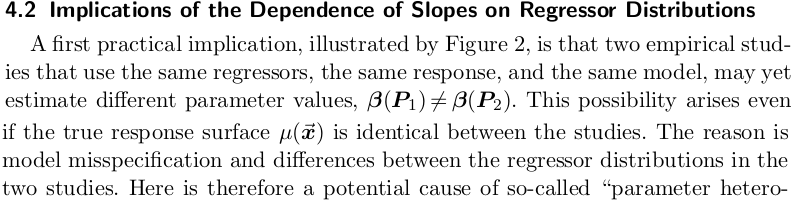
\includegraphics[width=.9\linewidth]{./quotes/sect4-implication.png}
\end{center}

\begin{center}
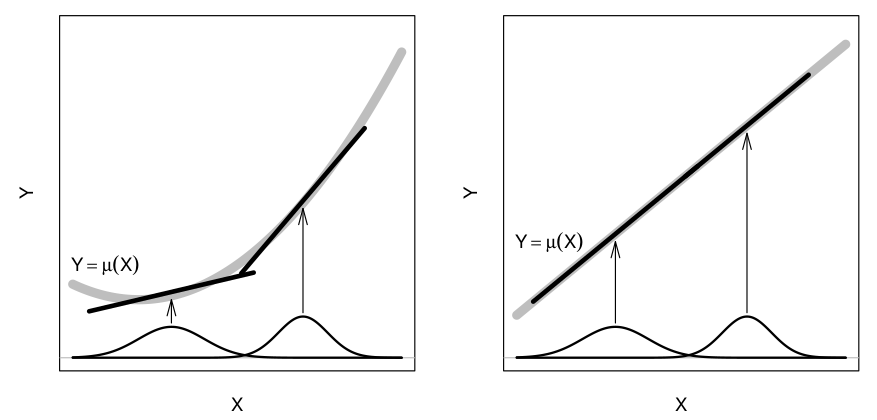
\includegraphics[width=.9\linewidth]{./quotes/sect4-fig2.png}
\end{center}
\end{frame}

\begin{frame}[label={sec:orgceb4262}]{Is this a problem?}
This seems to only be a problem because we do not understand how to interpret \(\beta(P)\).

\begin{block}{Average treatment effect (ATE)}
The ATE, \[\E[Y^1 - Y^0] = \E_P{[ \E_P[Y \mid X, A=1] - \E_P[Y \mid X, A=0]]}, \] should naturally
depend on the background distribution of \(X\).
\end{block}

\begin{block}{Conditional average treatment effect (CATE)}
The CATE, \[ \E[Y^1 - Y^0 \mid X=x] = \E_P[Y \mid X=x, A=1] - \E_P[Y \mid X=x, A=0], \] would not
depend on the background distribution \(X\) (right?).
\end{block}
\end{frame}

\begin{frame}[label={sec:orgf68d89c}]{Interpretation of ``slopes'' in the presence of non-linearity}
\begin{onlyenv}<1>
\begin{center}
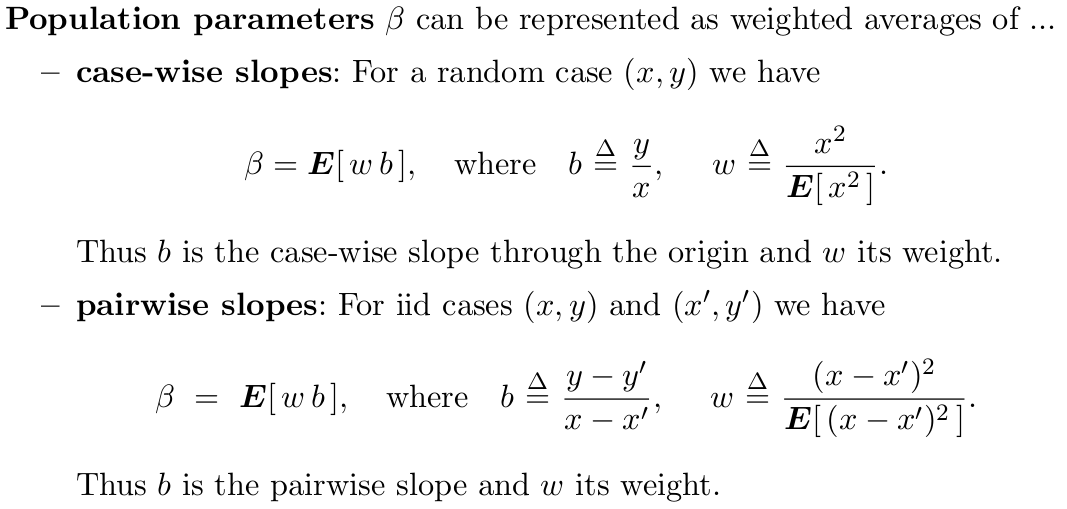
\includegraphics[width=.9\linewidth]{./quotes/sect10-interpretation.png}
\end{center}
\end{onlyenv}

\begin{onlyenv}<2>
\begin{center}
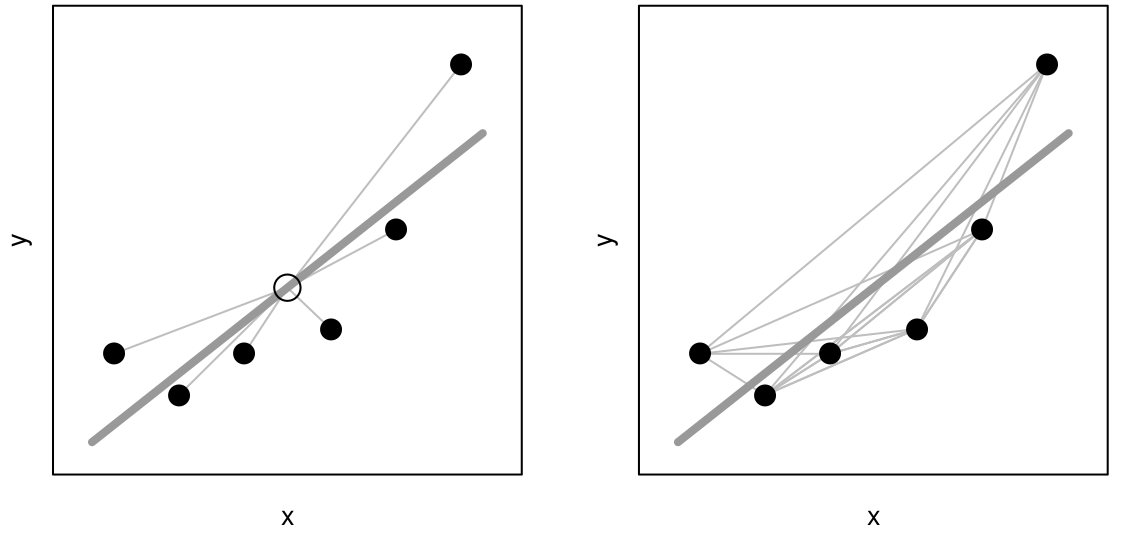
\includegraphics[width=.9\linewidth]{./quotes/sect10-figure.png}
\end{center}

\begin{center}
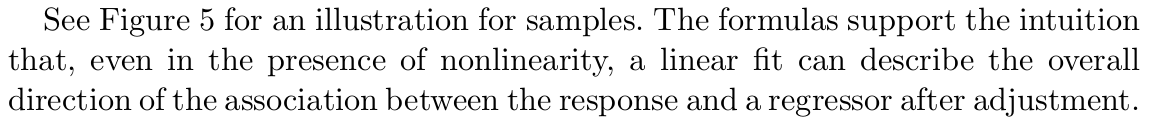
\includegraphics[width=.9\linewidth]{./quotes/sect10-interpretation-text.png}
\end{center}
\end{onlyenv}
\end{frame}

\section{Discussion papers}
\label{sec:org04ddf71}
\begin{frame}[label={sec:org4a90df8}]{Comments}
\end{frame}
\begin{frame}[label={sec:orgc991396}]{The best approximation depends on how you measure}
\begin{quote} %% 
In the context of prediction, the objective is often to minimize a particular criterion or scoring
rule. \ldots{} [In the] case of misspecification, it is not clear which criterion should be used for
estimation. In the context of forecasting conditional probabilities of binary outcomes, Elliott,
Ghanem and Krüger (2016) examine this question and illustrate that \alert{the choice of scoring rule
yields different best approximations to the true conditional probability function of the outcome of
interest under misspecification}, except under restrictive conditions. \citep{ghanem2019discussion}
\end{quote}
\end{frame}

\begin{frame}[label={sec:orgc4ffb0b}]{Predictive performance}
\cite{rinaldo2019comment} argue that we should give up the parameter \(\beta\) and instead consider:

\begin{block}{Proper causal effect}
\(\beta\) is often mis-interpreted as a causal quantity effect. Drop the parameter \(\beta\) and instead
define a causal quantity of interest rigorously using counterfactuals, SEMs, DAGs.
\end{block}

\begin{block}{Variable importance measure}
Non-parametric variable importance measures defined without reference to a model, for instance
proportion of variance explained or Shapley values.
\end{block}
\end{frame}

\begin{frame}[label={sec:org97f733b}]{The best approximation is ill-defined when data is coarsened}
\begin{center}
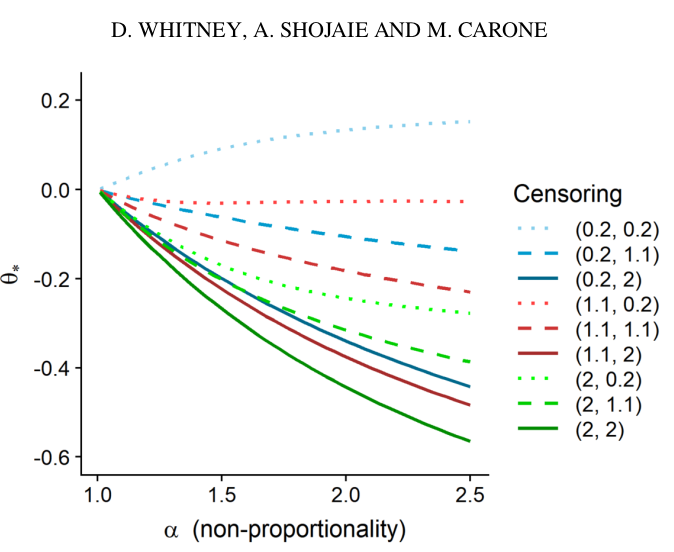
\includegraphics[width=7cm]{./quotes/comment-whitney-figure.png}
\end{center}

\begin{quote} %% 
\alert{The fact that the censoring distribution defines the estimand is particularly alarming}. In
commenting on this finding, O’Quigley (2008) states that the partial likelihood-based regression
functional is not itself particularly useful nor interpretable -- we agree with this viewpoint.
\citep{whitney2019comment}
\end{quote}
\end{frame}

\section{Additional thoughts}
\label{sec:org9206982}
\begin{frame}[label={sec:org63fc183}]{Fully non-parametric (model-free) parameter definition}
\begin{block}{Model \(\rightarrow\) parameter (more or less interpretable)}
Extend parameter from linear (or other) model to general (non-parametric) setting. The parameter
interpretation simplifies to well-known quantity when the model is correct
\citep{buja2019models,buja2019models2}.
\end{block}

\begin{block}{Interpretable parameter \(\rightarrow\) estimation by using model}
Define parameter of interest directly on the non-parametric family of probability measure --
model-agnostic/model-free parameter \citep{rinaldo2019comment,whitney2019comment}. Separates
parameter definition and estimation completely.
\end{block}
\end{frame}

\begin{frame}[label={sec:orge2ded2d}]{Flawed models as a fact of life?}
Back to the main paper: In practice we are going to use some kind of estimation and approximation.
\begin{center}
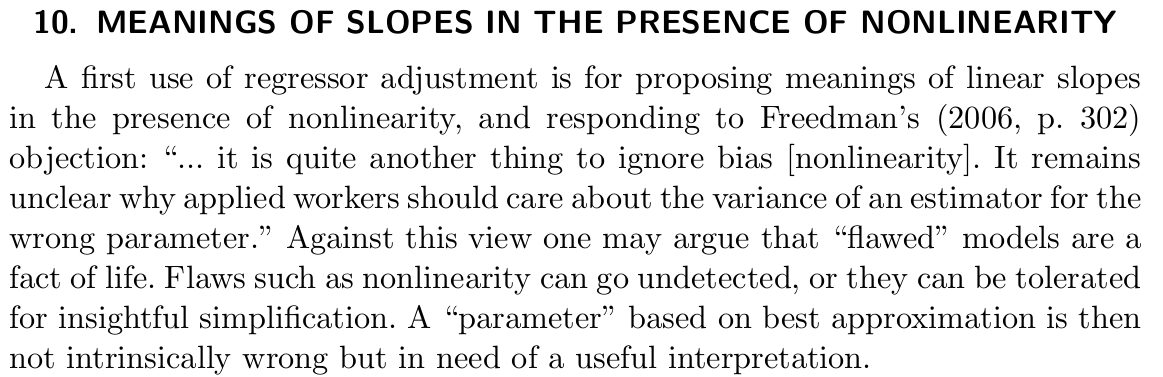
\includegraphics[width=.9\linewidth]{./quotes/sect10-model-approx.png}
\end{center}

The effect of estimating the nuisance parameter with an approximate nuisance model on the estimator
of a \emph{target parameter}:
\begin{itemize}
\item Assume the parameter of interest \(\Psi\) is identified through the nuisance parameter \(\nu\), i.e.,
\(\Psi(P) = \tilde\Psi(\nu(P))\).
\item If \(\hat \nu\) is an estimator of \(\nu\), then what effect does mis-specification/approximation for
the nuisance component have on the plug-in estimator \(\hat \Psi = \tilde\Psi(\hat \nu)\)?
\end{itemize}
\end{frame}

\begin{frame}[label={sec:orgc8e94cd}]{\normalsize Illustration of the effect of approximate nuisance model on target estimator}
\begin{block}{$\;$}
\small Estimation of the ATE using the G-formula. For the correctly specified outcome model (blue)
and a collection of mis-specified models indexed by a penalty parameter (red).

\begin{center}
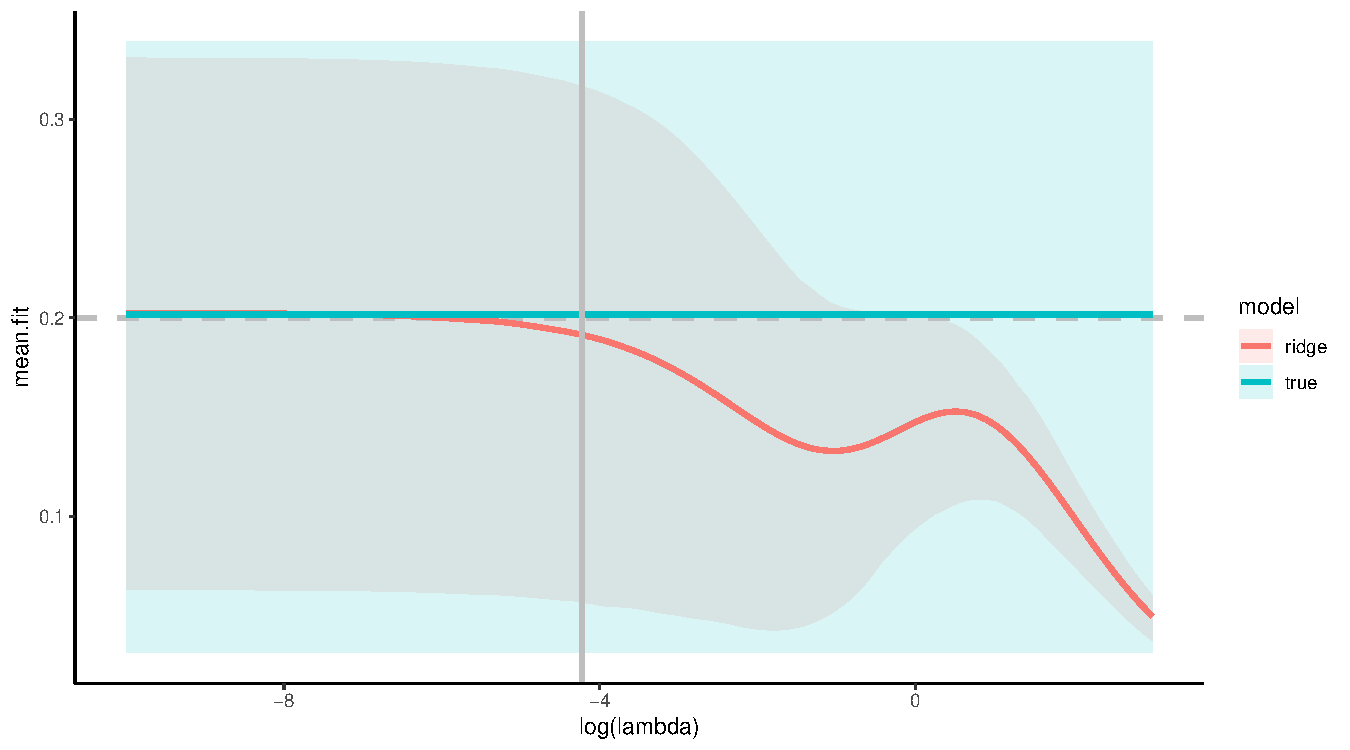
\includegraphics[width=.9\linewidth]{./fig-approximate-nuisance.pdf}
\end{center}
\end{block}
\end{frame}

\section{References}
\label{sec:org65b8d50}

\begin{frame}[label={sec:orge483fad}]{References}
\small \bibliography{/home/amnudn/Documents/latex/default-bib.bib}
\end{frame}
\end{document}